\chapter{Control Transfer}
\label{ch:control-transfer}

Most instructions continue with the next instruction in memory. Control-
transfer instructions make another future possible. A conditional branch asks
a question about the current state and chooses one of two addresses. A jump
selects a destination without asking. A call also leaves behind an address
from which execution can later continue.

These operations are small enough to fit in one line of assembly, yet they
connect nearly every part of the machine model. Their predicates read
registers or condition state. Their targets depend on instruction addresses,
lengths, and signed displacements. Their repeated execution makes loops. A
single error in the target convention can preserve every data result in a
one-step test and still send the program into the wrong block.

\begin{keyidea}[title={Control flow is arithmetic over addresses plus a predicate}]
A direct conditional branch needs three facts: the address used as its base,
the signed displacement or absolute destination, and the Boolean predicate
that selects the target instead of the fallthrough address. State all three
before proving where execution goes.
\end{keyidea}

\section{Why programs learned to choose}

The earliest stored-program machines already needed more than a straight
list of arithmetic operations. Repetition made a short program perform a long
calculation. Conditional transfer let that repetition stop when a counter,
remainder, or comparison reached the desired state. Subroutines then made one
piece of code serve many callers. The program counter turned stored
instructions from a static list into a path selected during execution.

Modern machines retain that foundation even when processors predict several
paths, fetch ahead, or execute instructions out of order. Architectural
semantics describe the committed path. A proof about a scalar instruction
set therefore needs no branch predictor, but it cannot omit the program
counter, the branch predicate, or the possibility of a bad target.

Control transfer serves several present-day purposes:

\begin{enumerate}
\item a conditional statement chooses between two computations;
\item a loop returns to a test or body;
\item a jump enters another block without creating a return link;
\item a call records a continuation address and enters a procedure;
\item an indirect transfer obtains its destination from a register or memory;
\item a trap or return crosses a boundary whose rules exceed ordinary scalar
control flow.
\end{enumerate}

This chapter handles direct conditional branches, direct jumps, and the link
values needed to prepare for procedures. Chapter 10 adds stacks and calling
agreements. Indirect calls, privilege changes, exceptions, and speculation
remain outside the present model unless a later section names them.

\begin{archive}[title={A loop compresses time into an address}]
A backward edge says that the same finite instruction bytes may act on a new
state. The code need not grow with the number of iterations. What grows is the
trace: one state after another, each justified by the same small transition
rules.
\end{archive}

\section{Fallthrough, target, and link}

Suppose an instruction begins at address \(p\) and occupies \(L\) bytes. Its
\keyterm{fallthrough address} is
\[
  f=p+L.
\]
Execution continues there when an ordinary instruction completes or a
conditional branch is not taken. For a direct relative transfer, a signed
displacement \(d\) is combined with a specified base \(b\):
\[
  t=b+d.
\]
The architecture decides whether \(b\) is the current instruction address,
the fallthrough address, or another quantity, and whether the encoded
displacement is scaled before addition.

For a predicate \(P(S)\) over state \(S\), the next program counter is
\[
 pc'=\left\{\begin{array}{ll}
 t & \hbox{when }P(S),\\
 f & \hbox{when }\neg P(S).
 \end{array}\right.
\]
A direct jump uses the first line without a predicate. A linking jump also
writes a \keyterm{link value}, normally an address at which a later return can
resume. The link is an architectural data result, not merely an annotation on
the control-flow graph.

\begin{figure}[htbp]
\centering
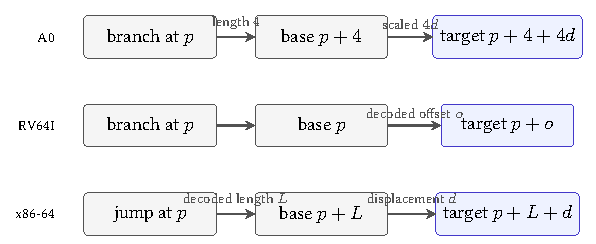
\includegraphics[width=0.94\textwidth]{figures/relative-target-conventions}
\caption{Three selected relative-target conventions. Similar assembly
displacements do not imply the same base, scale, or instruction length.}
\figalt{A0 branches from pc plus 4 using a scaled displacement, RV64 branches from pc, and x86 jumps from the following instruction.}
\label{fig:relative-target-conventions}
\end{figure}

Figure~\ref{fig:relative-target-conventions} exposes a common source of
off-by-one-instruction errors. A0 deliberately uses \(p+4+4d\). Selected
RV64I conditional branches add their sign-extended, encoded offset to the
address of the branch instruction. Selected x86-64 relative jumps add a
sign-extended displacement to the instruction pointer for the following
instruction. RV64I instructions in this chapter are four bytes, while the
x86-64 instruction length depends on the actual encoding. The source-pinned
rules appear in the RISC-V unprivileged specification and Intel instruction
reference \autocite{riscv2026unpriv,intel2026sdm2}.

\begin{warning}[title={Never infer the target base from the printed operand}]
An assembler may print a destination label, a byte displacement, or a
symbolic expression. The architectural rule operates on encoded fields and a
defined program-counter base. Decode the instruction and name that base before
doing target arithmetic.
\end{warning}

\begin{example}[title={The same address, three calculations}]
Place a transfer at address 100. An A0 branch with encoded displacement 3
targets \(100+4+4(3)=116\). An RV64I branch whose decoded offset is 16 bytes
targets \(100+16=116\). An x86-64 near conditional jump of length 6 with
displacement 10 targets \((100+6)+10=116\). All three reach the same address,
but no pair uses identical encoded numbers and conventions.
\end{example}

\begin{proofkit}[title={A target calculation that survives relocation}]
Let an instruction and its target both move by the same address delta \(k\).
If the relative displacement is target minus the architecture's base, that
base also moves by \(k\). The new displacement is
\((t+k)-(b+k)=t-b\). Thus the encoded relative distance is unchanged, provided
the moved target remains representable and alignment and encoding constraints
still hold. The cancellation explains why relative branches help relocatable
code; it does not prove that every relocation stays in range.
\end{proofkit}

\section{A0 makes both edges explicit}

A0 instructions are four bytes and begin at four-byte-aligned addresses. An
ordinary instruction advances from \(p\) to \(p+4\). A conditional branch with
signed eight-bit immediate \(d\) selects \(p+4+4d\) when its condition is true
and \(p+4\) otherwise. The scale of four ensures that a target obtained from
an aligned branch is aligned. It does not ensure that the target contains a
complete legal instruction; fetch and decode still have to succeed.

A0 supplies eight branch predicates over \(Z,N,C,V\). Equality and inequality
read \(Z\). Signed less-than and greater-than-or-equal test whether \(N\) and
\(V\) differ or agree. Unsigned lower and higher conditions use the no-borrow
bit \(C\), with \(Z\) distinguishing strict from non-strict comparisons. The
branch preserves registers, memory, and conditions. Its visible write is the
program counter, unless the selected target causes a later fetch trap.

Consider this width-eight loop, with each line occupying four bytes:

\begin{codelisting}[language={},caption={A0 counts r0 down to zero}]
00: movi r1, 1
04: cmp  r0, r1
08: branch.lo exit
0c: sub  r0, r0, r1
10: branch.ne loop
14: halt
\end{codelisting}

The first comparison protects the subtraction when the initial unsigned value
is zero. For a positive initial \(r_0\), subtraction decreases the unsigned
reading by one without wrapping. The subtraction also updates \(Z\), so
\code{branch.ne} returns to the loop body exactly while the result is nonzero.
The listing uses labels for reading; an encoder must replace them with signed
displacements that satisfy A0's target formula.

\begin{tryit}[title={Encode both A0 branch displacements}]
Using the addresses in the listing, let \code{exit} denote address 20 and
\code{loop} denote address 12. Solve \(p+4+4d=t\) for each branch. Check that
both signed values fit in byte 3, then recompute the destinations from the
encoded values.
\end{tryit}

The branch at address 8 needs \(d=2\), because \(8+4+4(2)=20\). The backward
branch at address 16 needs \(d=-2\), because \(16+4+4(-2)=12\). Treating the
current address rather than the fallthrough address as the base would send
both branches four bytes early.

\section{RV64I compares registers at the branch}

The selected RV64I conditional branches compare two integer registers as part
of the branch instruction. \code{BEQ} and \code{BNE} test equality.
\code{BLT} and \code{BGE} use signed readings; \code{BLTU} and \code{BGEU}
use unsigned readings. A taken branch adds its decoded, sign-extended B-type
offset to the address of the branch instruction. An untaken branch proceeds
to the following instruction \autocite{riscv2026unpriv}.

\begin{codelisting}[language={},caption={RV64I counts a0 down to zero}]
    beq  a0, x0, exit
loop:
    addi a0, a0, -1
    bne  a0, x0, loop
exit:
\end{codelisting}

Here \code{x0} supplies the constant zero. The branch itself reads both named
registers. The \code{addi} instruction changes \code{a0} but creates no
x86-style zero flag; \code{bne} performs the next comparison directly.
Assembler register names such as \code{a0} carry ABI meaning, while the base
ISA semantics identify an integer register. Chapter 10 separates those two
layers.

RV64I also provides direct jumps with links. \code{JAL rd,offset} writes the
address of the following instruction to \code{rd} and transfers to a
PC-relative target. Writing the link to \code{x0} discards it and yields a
plain direct jump. \code{JALR} obtains a target from a register plus immediate,
writes a link, and clears the target's low bit under its architectural rule.
The direct loop above needs neither instruction, but procedures will.

\begin{sidebar}[title={A pseudoinstruction is not another semantic primitive}]
An assembler may print \code{j label}, \code{ret}, or a branch-against-zero
mnemonic that expands to a base instruction. Proofs over machine code must use
the decoded base instruction and its operands. Pseudoinstructions remain
valuable explanations of programmer intent, but they do not add encodings.
\end{sidebar}

The conditional-branch immediate is assembled from noncontiguous instruction
bits and has alignment constraints. A chapter proof may begin with the decoded
offset when encoding is not under study, but the evidence manifest must say so.
A decoder theorem and a step theorem are different claims: the first recovers
the offset; the second uses it to update the program counter.

\section{x86-64 reads flags and counts variable-length bytes}

Selected x86-64 compare instructions perform a subtraction for flags without
storing the arithmetic result. A following \code{Jcc} reads the condition
formula associated with its suffix. For example, \code{JE} reads ZF;
\code{JNE} reads its negation; signed less-than uses \(SF\ne OF\); and
unsigned below uses CF. The exact flag effects and accepted encodings belong
to the selected instruction forms in Intel's reference, not to the mnemonic
name in isolation \autocite{intel2026sdm2}.

\begin{codelisting}[language={},caption={x86-64 counts RDI down to zero}]
    test rdi, rdi
    je   exit
loop:
    sub  rdi, 1
    jne  loop
exit:
\end{codelisting}

\code{test rdi,rdi} computes a bitwise conjunction for flags and leaves
\code{rdi} unchanged. It sets ZF exactly when the selected value is zero.
\code{sub} then decrements the register and supplies the ZF consumed by
\code{jne}. This dependency is real even though it is absent from the
register operands printed on the jump.

x86-64 relative jump targets use the instruction pointer for the following
instruction as their base. Because instruction lengths vary, the decoder must
first determine that next address. Short and near conditional-jump encodings
can express different displacement widths while implementing the same
predicate. Replacing one encoding with another changes instruction length and
therefore changes both the base and the displacement required for a fixed
destination.

\begin{warning}[title={A flag-reading jump has a hidden-looking input}]
The condition suffix identifies which flags the jump reads. Register equality
at the jump is irrelevant unless preceding instructions established the
required flags. Moving, replacing, or inserting a flag-writing instruction
between compare and jump can change the path without changing any explicit
jump operand.
\end{warning}

The x86-64 loop, the RV64I loop, and the A0 loop implement the same small
mathematical recurrence only under declared input and observation relations.
They do not have identical registers, instruction counts, condition state, or
program-counter values. A proof must relate those differences instead of
erasing them.

\section{Direct and indirect transfers owe different proofs}

A direct transfer carries a destination relative to the instruction or names
one through relocation. Once its bytes and address are fixed, target arithmetic
usually determines one destination. An \keyterm{indirect transfer} obtains at
least part of its destination from current machine state. The same instruction
bytes may therefore reach many addresses on different executions.

This difference changes the proof. For a direct branch, faithful decode and
correct target arithmetic can identify the destination locally. For an
indirect jump, local instruction semantics only explain how a register or
memory value becomes a candidate program counter. A surrounding invariant must
restrict that value to an allowed target set. A compiler might derive the set
from a switch table, a procedure proof from a saved continuation, or a
control-flow integrity policy from approved entry points.

\begin{figure}[htbp]
\centering
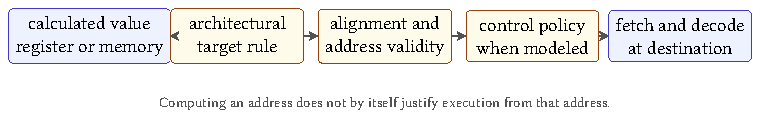
\includegraphics[width=0.96\textwidth]{figures/indirect-target-gates}
\caption{An indirect destination passes through several proof gates before the
next instruction may be justified. Some machines omit or add policy gates, but
the target value alone is never the whole argument.}
\figalt{A calculated register or memory value passes through an architectural target rule, address validity, optional control policy, and destination fetch and decode.}
\label{fig:indirect-target-gates}
\end{figure}

RV64I \code{JALR}, for example, adds a sign-extended immediate to a register
value and clears the least significant bit of the result. A theorem must use
that transformed target rather than equating the new program counter with the
raw register. Selected x86-64 indirect branches obtain their destinations from
register or memory operands under their own mode and operand rules. Core A0
has no indirect jump, so a proof must not manufacture one from a register that
happens to contain an address.

Target validity is a second question. Depending on the model, the destination
may need suitable alignment, a canonical address, mapped executable memory,
an instruction boundary, and bytes that decode legally. A hardware or
operating-system policy may add another restriction. These checks need not all
occur in the transfer instruction itself. A model may update the program
counter first and report a fetch failure on the next step. The trace should
preserve that ordering instead of replacing it with one generic failure.

\begin{warning}[title={A finite target set needs provenance}]
Listing the destinations seen in tests does not establish the allowed target
set. Derive the set from a table bound, type invariant, saved-link contract, or
other stated premise. Then show that every calculated destination belongs to it
and that every member is a valid entry under the selected semantics.
\end{warning}

Return instructions are important indirect transfers. Their intended target
comes from a prior call, but that history is not automatic evidence. The proof
must connect the current link register or stacked word to the continuation
created at the matching call and show that intervening execution preserved it.
Chapter 10 turns that historical connection into a procedure contract.

\begin{definition}[title={Target soundness and target completeness}]
For an indirect transfer under a precondition, target soundness says that every
destination the machine can select belongs to the declared target set. Target
completeness says that every destination claimed as possible can actually be
selected by some allowed entry state. Soundness protects execution from an
omitted bad destination. Completeness prevents a coarse analysis from adding
spurious edges that may obscure invariants or make a later proof needlessly
hard.
\end{definition}

The two directions need different witnesses. A soundness failure is one entry
state whose selected destination lies outside the set. A completeness claim
needs, for each listed destination, an allowed state that reaches it. Many
safety arguments require soundness but not completeness. An exact
control-flow graph requires both, which is why a graph inferred from a few
runs is generally neither a safe overapproximation nor an exact account.

\section{One loop, three state shapes}

Let the input be a nonnegative mathematical integer \(n\) that fits in the
selected word without wrapping during the loop. Each program maintains a
machine word whose unsigned reading is the number of decrements remaining.
The common control-flow graph has an entry test, a decrementing body, a back
edge, and an exit.

\begin{figure}[htbp]
\centering
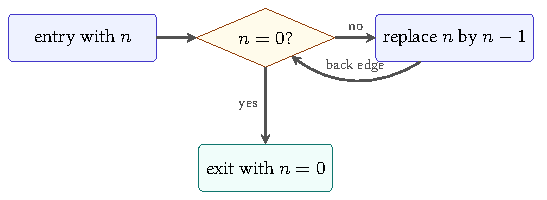
\includegraphics[width=0.82\textwidth]{figures/counted-loop-graph}
\caption{The common mathematical control shape beneath the three listings.
The machine-specific predicates and target conventions implement these edges.}
\figalt{Entry tests n equals zero, the body replaces n by n minus one, a back edge repeats, and zero exits.}
\label{fig:counted-loop-graph}
\end{figure}

At the head of the body, use the invariant
\[
  0 < \langle r\rangle_u \leq n,
\]
where \(r\) denotes the machine's related counter register. The body changes
the reading from \(k>0\) to \(k-1\). The value therefore remains in range and
strictly decreases as a natural number. When it becomes zero, the back-edge
predicate is false and execution reaches the exit.

\begin{proofkit}[title={Termination and final value of the counted loop}]
If the input is zero, the entry test reaches the exit without executing the
body. Otherwise let the counter reading at the first body entry be \(n>0\).
Each body execution subtracts one from a positive reading, so modular
subtraction agrees with natural subtraction and cannot wrap. The natural
measure decreases from \(n\) through \(n-1,\ldots,1,0\). A strictly decreasing
natural measure cannot decrease forever. At zero, each machine's related
not-equal predicate is false, so the program exits with counter value zero.
\end{proofkit}

The premise that subtraction occurs only at a positive value is load-bearing.
Delete the entry test and start at zero: fixed-width subtraction produces the
maximum unsigned word, after which the loop may take \(2^w-1\) further
iterations before returning to zero. The original termination conclusion may
still hold for a finite width, but the proof, trace length, and intended cost
claim have changed.

The invariant is also not a complete cross-ISA relation. Such a relation must
identify A0 \(r_0\), RV64I \code{a0}, and x86-64 \code{RDI}; relate the values
at chosen control points; state what memory must agree on; map A0's \(Z\) and
x86-64's ZF when their branches depend on them; and permit the RV64I state to
lack that flag. Chapter 12 develops this style of relation.

\begin{goingdeeper}[title={Stuttering between related control points}]
One machine may need an extra compare or test instruction before a branch.
The other may combine comparison and transfer. A simulation can relate states
only at loop heads and exits, allowing several steps on one side for one or
several on the other. This is stuttering, not an error, provided the relation
is restored at the declared observation points.
\end{goingdeeper}

\subsection{Safety, progress, and termination are separate}

The counted-loop argument combines three claims that should remain visible.
\emph{Safety} says every visited instruction and memory access is defined and
the subtraction does not wrap under the intended natural-number reading.
\emph{Progress} says a nonterminal state can take another justified step.
\emph{Termination} says the run eventually reaches the exit. A decreasing
natural measure helps with termination only after safety and progress connect
each iteration to the next loop head.

The separation becomes useful when a proof fails. A counter may decrease on
every completed iteration while an invalid branch target traps before the next
head. The measure argument is then true but irrelevant to normal termination.
A loop may remain safe forever while its measure fails to decrease. Or it may
reach the exit with the expected counter while corrupting an observed memory
location. No one of these facts substitutes for the others.

Iteration count is another conclusion, not a side effect of termination. Add a
ghost natural number \(i\) counting completed decrements and strengthen the
invariant at the loop head to
\[
  i+\langle r\rangle_u=n.
\]
Initially \(i=0\) and the counter reads \(n\). One body step increases \(i\) by
one and decreases the counter reading by one, preserving the sum. At exit the
counter is zero, so \(i=n\). The ghost value is proof bookkeeping; it need not
exist in machine state.

\begin{proofkit}[title={Why the variant must be checked at one control point}]
A variant can rise inside an iteration and still decrease from one loop head
to the next. Choose a recurring control point, prove that every return to it
has a smaller natural variant, and prove that execution cannot avoid either
that return or an exit forever. Comparing values at arbitrary adjacent
instructions can reject correct loops or accept a cycle that bypasses the
measurement point.
\end{proofkit}

\section{From traces to control-flow claims}

A trace records the actual successor at each step. For a chosen input, a
checker can decode the instruction at the recorded program counter, recompute
its predicate and target, and compare the complete successor with the next
state in the trace. This catches a wrong edge, a wrong decrement, a stale
condition bit, or execution after a terminal outcome.

One trace does not prove a general loop theorem. Running the loop from inputs
zero through 255 proves facts about those chosen executions under a trusted
enumeration and checker. The invariant proof covers every input in its stated
domain because it reasons about an arbitrary positive counter and a decreasing
measure. Machine evidence can support that argument by checking the step
lemmas or refuting their negations, but a bounded replay cannot silently
become an unbounded theorem.

\begin{definition}[title={A bounded run has three distinct endings}]
A bounded interpreter may halt, trap, or exhaust its step bound while the
machine is still running. Bound exhaustion is not a machine trap and not proof
of nontermination. It says only that this run prefix did not reach a terminal
outcome within the supplied budget.
\end{definition}

A control-flow graph also differs from a trace. The graph contains possible
edges admitted by local branch analysis. A trace contains the one edge
selected in each visited state. Proving that an edge is unreachable needs a
state argument, not merely its absence from a few traces.

The graph can be checked at several strengths. A syntactic graph connects each
decoded direct transfer to its calculated destination and adds fallthrough
where appropriate. An indirect edge may conservatively point to many possible
targets. A state-restricted graph removes edges whose predicates or target
values are impossible under a supplied invariant. Reachability from the entry
then removes disconnected code. Each reduction needs evidence: a visually
tidy graph is not a proof that the omitted edge cannot execute.

Loops arise from cycles in this reachable graph, but a cycle alone does not
identify an induction invariant or termination measure. Conversely, an
unrolled trace can revisit an address without revealing every possible cycle.
Graph structure organizes the proof obligations; semantic reasoning over
states discharges them.

\section{An introductory Axeyum route}

The current Axeyum checkout supplies reusable bit-vector, solver,
certificate, and kernel components. It does not yet supply executable A0,
RV64I, or x86-64 instruction semantics. For this chapter, Axeyum use is
therefore a construction route with a precise boundary, not a claim that the
three loops already run there.

Start with A0 because its complete state and fixed-width encoding are owned by
this book. Define a decoded branch containing a condition code and signed
displacement. Define the predicate as a pure function of \(Z,N,C,V\), then
define the two successor-PC formulas. Only after unit tests cover every
condition and both outcomes should the branch enter the general A0 step
function.

The first evidence object should contain an initial state, instruction bytes,
decoded branch, selected predicate value, expected successor state, and the
semantic-package digest. Its checker should decode again and recompute the
step rather than trusting recorded derived fields. A small command-line
wrapper can then print a teaching trace while its exit status depends on full
agreement.

\begin{example}[title={Controls for the first branch checker}]
Use a positive case whose taken target differs from fallthrough. Pair it with
mutations that invert the predicate, omit the displacement scale, use \(pc\)
instead of \(pc+4\) as the A0 base, or change one reserved encoding bit. Each
mutation must make the checker fail for the intended reason. Also retain a
valid untaken case so a checker that always chooses the target cannot pass.
\end{example}

The RV64I and x86-64 routes come later. Each needs a source-pinned decoder
slice before its transition function can carry machine-code claims. The RV64I
control should mutate a split immediate field or confuse signed and unsigned
predicates. The x86-64 control should alter a prefix, opcode, displacement, or
decoded length. A handwritten branch formula can test arithmetic; it cannot
stand in for those decoders.

For the counted-loop theorem, separate four evidence levels:

\begin{enumerate}
\item replay one complete trace for a small input;
\item enumerate every input at a teaching width;
\item ask for a counterexample to invariant preservation at a named width and
replay any model;
\item reconstruct a width-parametric decreasing-measure proof through a
kernel route when that route exists.
\end{enumerate}

The manifest must label which level was achieved. Solver \code{UNSAT} at
width 64 is a strong finite-width result, but it is not automatically a theorem
quantified over every positive width. A proof certificate can reduce trust in
the solver verdict; it still proves only the encoded formula.

\section{What a branch proof must establish}

Branch correctness is often compressed into the phrase ``the target is
right.'' That phrase hides several separate obligations. Keeping them separate
makes both reader proofs and negative controls more useful.

First comes \emph{fetch and decode}. The current program counter must identify
a complete legal instruction. The decoder must recover the intended condition,
register fields, and signed displacement. A proof that starts from an already
decoded branch may assume this layer, but it must say so.

Second comes \emph{predicate agreement}. The implementation must ask the
question named by the instruction. Signed and unsigned comparisons can choose
different edges for the same word pair. A0 and selected x86-64 forms must read
the condition state produced by the preceding instruction; an RV64I branch
must read the specified register values. Preserving the right target while
inverting the predicate is still a wrong branch.

Third comes \emph{target arithmetic}. The proof must identify the base,
extension rule, scale, and arithmetic width. It must also distinguish the
taken target from fallthrough. Alignment, canonical-address, and mapped-code
requirements belong here when the selected machine model includes them.

Fourth comes \emph{state preservation}. A conditional branch usually changes
the program counter and preserves most other architectural state. ``Reached
the right block'' does not justify an unnoticed register, memory, flag, or
outcome change. A linking jump is different because its link destination is an
intended additional write.

Finally comes \emph{context}. The successor address must lead to code whose
execution is covered by the surrounding claim. A locally correct edge into an
illegal byte sequence traps on the next step. A locally correct loop edge does
not prove termination. Those are composition properties beyond the branch's
single transition.

\begin{proofkit}[title={Five obligations for a direct conditional branch}]
Check, in order: legal fetch and faithful decode; the exact predicate over the
declared input state; taken and untaken program-counter formulas; preservation
of every other observed component; and the premise needed to continue from
the chosen successor. A proof may discharge the layers separately, but the
whole-program claim needs all five.
\end{proofkit}

This decomposition locates counterexamples. A wrong immediate field is a
decode failure. A stale ZF is a predicate failure. A missing A0 scale factor is
a target failure. A jump that clears an unrelated register is a preservation
failure. A correct backward edge in a loop without a decreasing measure is a
context failure. Merely reporting that ``the branch test failed'' throws away
the lesson carried by the witness.

\section{Where the control model stops}

This chapter treats architectural steps as atomic and sequential. It excludes
branch prediction, speculative execution, pipeline recovery, timing, caches,
and side channels. Those mechanisms can make two architecturally equivalent
paths observably different to a timing adversary, but they require another
state and observation model.

We also exclude interrupts, exceptions beyond A0's declared traps, privilege
transfers, self-modifying code, concurrent modification, and weak memory.
Indirect control flow receives only the link and target facts needed for the
next chapter. A full account must also specify target validity, canonical
addresses, control-flow enforcement, and the memory from which an indirect
destination may be loaded.

Within the boundary, the central fact is exact and surprisingly broad. A
finite program becomes an indefinitely extensible process because the program
counter may revisit an address. The mystery does not lie in an unspecified
machine. It lies in the consequence of a rule small enough to write on one
line: choose a successor, then apply the same semantics again.

\section{Exercises}

\begin{enumerate}
\item \textbf{Execute.} Trace both outcomes of an A0 \code{branch.eq} at
address 40 with displacement \(-3\). Give the successor program counter and
all preserved state components.

\item Compute the A0 displacement needed to branch from addresses 0, 12, and
100 to address 40. State which values fit the signed byte and which targets
meet the alignment rule.

\item \textbf{Break.} Replace A0's taken-target rule \(pc+4+4d\) with
\(pc+4d\). Give a branch for which the mutation accidentally agrees and one
for which it reaches a different legal instruction.

\item A four-byte RV64I branch lies at address 100 and has decoded offset
\(-20\). A six-byte x86-64 near jump lies at address 100 and has displacement
\(-20\). Compute both targets and explain the difference.

\item Explain why changing an x86-64 conditional jump from a short encoding
to a longer encoding requires displacement repair even when its address and
destination label appear unchanged.

\item For each A0 predicate \code{eq}, \code{lt}, \code{lo}, and \code{hi},
give values of \(Z,N,C,V\) that take and do not take the branch. Identify
condition combinations that cannot arise from one selected comparison, if
your claim assumes such a comparison.

\item Rewrite the RV64I counted loop to count upward from zero to an input
bound. State whether its comparison is signed or unsigned and give an input
premise that prevents wraparound.

\item \textbf{Prove.} Strengthen the counted-loop invariant to say exactly
how many body executions have occurred. Use it to prove both final value and
iteration count.

\item Delete the entry test from each loop and start the counter at zero at
width four. Trace enough steps to identify the new iteration count. Explain
why the original natural-number proof no longer applies at the first step.

\item \textbf{Transfer.} Define relation checkpoints for the three loop
listings. Map counter values, control locations, outcomes, and the condition
information required for the next branch; identify scratch or flag state that
the final observation may omit.

\item Give two instruction sequences that leave the same counter register but
different x86-64 flags immediately before \code{jne}. Supply initial values
for which the chosen edges differ.

\item Explain the difference among a trace, a control-flow graph, and a proof
that a graph edge is unreachable. Give one fact each can establish.

\item Design a bounded-run result type that distinguishes halt, trap, and
bound exhaustion. Give a negative test for an implementation that reports
bound exhaustion as nontermination.

\item Design the first A0 branch artifact for Axeyum. Include bytes, decoded
instruction, initial state, expected successor, semantic digests, checker
command, and four target or predicate mutations.

\item \textbf{Transfer.} State the obligations for replacing an A0
condition-reading branch with an RV64I register-comparing branch. Include the
state relation before the branch and the relation required after both taken
and untaken outcomes.
\end{enumerate}
